\documentclass[11pt]{article}

% NOTE: Add in the relevant information to the commands below; or, if you'll be using the same information frequently, add these commands at the top of paolo-pset.tex file. 
\newcommand{\name}{Agustin Esteva}
\newcommand{\email}{aesteva@uchicago.edu}
\newcommand{\classnum}{13110}
\newcommand{\subject}{SSI: Formal Theory}
\newcommand{\instructors}{Jingyuan Qian}
\newcommand{\assignment}{Problem Set 2}
\newcommand{\semester}{Fall 2024}
\newcommand{\duedate}{2024-10-11}
\newcommand{\bA}{\mathbf{A}}
\newcommand{\bB}{\mathbf{B}}
\newcommand{\bC}{\mathbf{C}}
\newcommand{\bD}{\mathbf{D}}
\newcommand{\bE}{\mathbf{E}}
\newcommand{\bF}{\mathbf{F}}
\newcommand{\bG}{\mathbf{G}}
\newcommand{\bH}{\mathbf{H}}
\newcommand{\bI}{\mathbf{I}}
\newcommand{\bJ}{\mathbf{J}}
\newcommand{\bK}{\mathbf{K}}
\newcommand{\bL}{\mathbf{L}}
\newcommand{\bM}{\mathbf{M}}
\newcommand{\bN}{\mathbf{N}}
\newcommand{\bO}{\mathbf{O}}
\newcommand{\bP}{\mathbf{P}}
\newcommand{\bQ}{\mathbf{Q}}
\newcommand{\bR}{\mathbf{R}}
\newcommand{\bS}{\mathbf{S}}
\newcommand{\bT}{\mathbf{T}}
\newcommand{\bU}{\mathbf{U}}
\newcommand{\bV}{\mathbf{V}}
\newcommand{\bW}{\mathbf{W}}
\newcommand{\bX}{\mathbf{X}}
\newcommand{\bY}{\mathbf{Y}}
\newcommand{\bZ}{\mathbf{Z}}
\newcommand{\Var}{\text{Var}}

%% blackboard bold math capitals
\newcommand{\bbA}{\mathbb{A}}
\newcommand{\bbB}{\mathbb{B}}
\newcommand{\bbC}{\mathbb{C}}
\newcommand{\bbD}{\mathbb{D}}
\newcommand{\bbE}{\mathbb{E}}
\newcommand{\bbF}{\mathbb{F}}
\newcommand{\bbG}{\mathbb{G}}
\newcommand{\bbH}{\mathbb{H}}
\newcommand{\bbI}{\mathbb{I}}
\newcommand{\bbJ}{\mathbb{J}}
\newcommand{\bbK}{\mathbb{K}}
\newcommand{\bbL}{\mathbb{L}}
\newcommand{\bbM}{\mathbb{M}}
\newcommand{\bbN}{\mathbb{N}}
\newcommand{\bbO}{\mathbb{O}}
\newcommand{\bbP}{\mathbb{P}}
\newcommand{\bbQ}{\mathbb{Q}}
\newcommand{\bbR}{\mathbb{R}}
\newcommand{\bbS}{\mathbb{S}}
\newcommand{\bbT}{\mathbb{T}}
\newcommand{\bbU}{\mathbb{U}}
\newcommand{\bbV}{\mathbb{V}}
\newcommand{\bbW}{\mathbb{W}}
\newcommand{\bbX}{\mathbb{X}}
\newcommand{\bbY}{\mathbb{Y}}
\newcommand{\bbZ}{\mathbb{Z}}

%% script math capitals
\newcommand{\sA}{\mathscr{A}}
\newcommand{\sB}{\mathscr{B}}
\newcommand{\sC}{\mathscr{C}}
\newcommand{\sD}{\mathscr{D}}
\newcommand{\sE}{\mathscr{E}}
\newcommand{\sF}{\mathscr{F}}
\newcommand{\sG}{\mathscr{G}}
\newcommand{\sH}{\mathscr{H}}
\newcommand{\sI}{\mathscr{I}}
\newcommand{\sJ}{\mathscr{J}}
\newcommand{\sK}{\mathscr{K}}
\newcommand{\sL}{\mathscr{L}}
\newcommand{\sM}{\mathscr{M}}
\newcommand{\sN}{\mathscr{N}}
\newcommand{\sO}{\mathscr{O}}
\newcommand{\sP}{\mathscr{P}}
\newcommand{\sQ}{\mathscr{Q}}
\newcommand{\sR}{\mathscr{R}}
\newcommand{\sS}{\mathscr{S}}
\newcommand{\sT}{\mathscr{T}}
\newcommand{\sU}{\mathscr{U}}
\newcommand{\sV}{\mathscr{V}}
\newcommand{\sW}{\mathscr{W}}
\newcommand{\sX}{\mathscr{X}}
\newcommand{\sY}{\mathscr{Y}}
\newcommand{\sZ}{\mathscr{Z}}


\renewcommand{\emptyset}{\O}

\newcommand{\abs}[1]{\lvert #1 \rvert}
\newcommand{\norm}[1]{\lVert #1 \rVert}
\newcommand{\sm}{\setminus}


\newcommand{\sarr}{\rightarrow}
\newcommand{\arr}{\longrightarrow}

% NOTE: Defining collaborators is optional; to not list collaborators, comment out the line below.
%\newcommand{\collaborators}{Alyssa P. Hacker (\texttt{aphacker}), Ben Bitdiddle (\texttt{bitdiddle})}

\input{paolo-pset.tex}

% NOTE: To compile a version of this pset without problems, solutions, or reflections, uncomment the relevant line below.

%\excludeversion{problem}
%\excludeversion{solution}
%\excludeversion{reflection}

\begin{document}	
	
	% Use the \psetheader command at the beginning of a pset. 
	\psetheader
\section*{Problem 1}
\begin{problem}
Prof. Zhaotian Luo, another political science professor, will be your instructor for
SSI Formal Theory III in the Spring Quarter. Consider the following statement:
\begin{quote}
“Zhaotian and Juan are both Chinese political scientists. If Juan is one of your
favorite Chinese people and Zhaotian is one of your favorite political scientists,
then Juan is also one of your favorite political scientists and Zhaotian is also one
of your favorite Chinese people.”
\end{quote}
\end{problem}
\begin{enumerate}
    \item 
    \begin{problem}
        Express the statement in formal language. Please use the choice set, $C()$ to denote someone being among your favorites.
    \end{problem}
    \begin{solution}
        Let 
        \begin{align*}
            z &:= \text{Zhaotian}\\
            j &:= \text{Juan}\\
            CP &:= \{\text{all Chinese political scientists}\}\\
            CH &;= \{\text{all Chinese people}\}\\
            PS &:= \{\text{all political scientists}\}
        \end{align*}
        Then we have the following statement:
        \begin{quote}
            Suppose $z\in CP$ and $j \in CP.$ Then if $j\in C(CH)$ and $z \in C(PS),$ then $j\in C(PS)$ and $z\in C(CH).$
        \end{quote}
    \end{solution}
    \item 
    \begin{problem}
        Use a Venn diagram, similar to the one on p.17, to represent this relationship.
    \end{problem}
    \begin{figure}[h!]
        \centering
        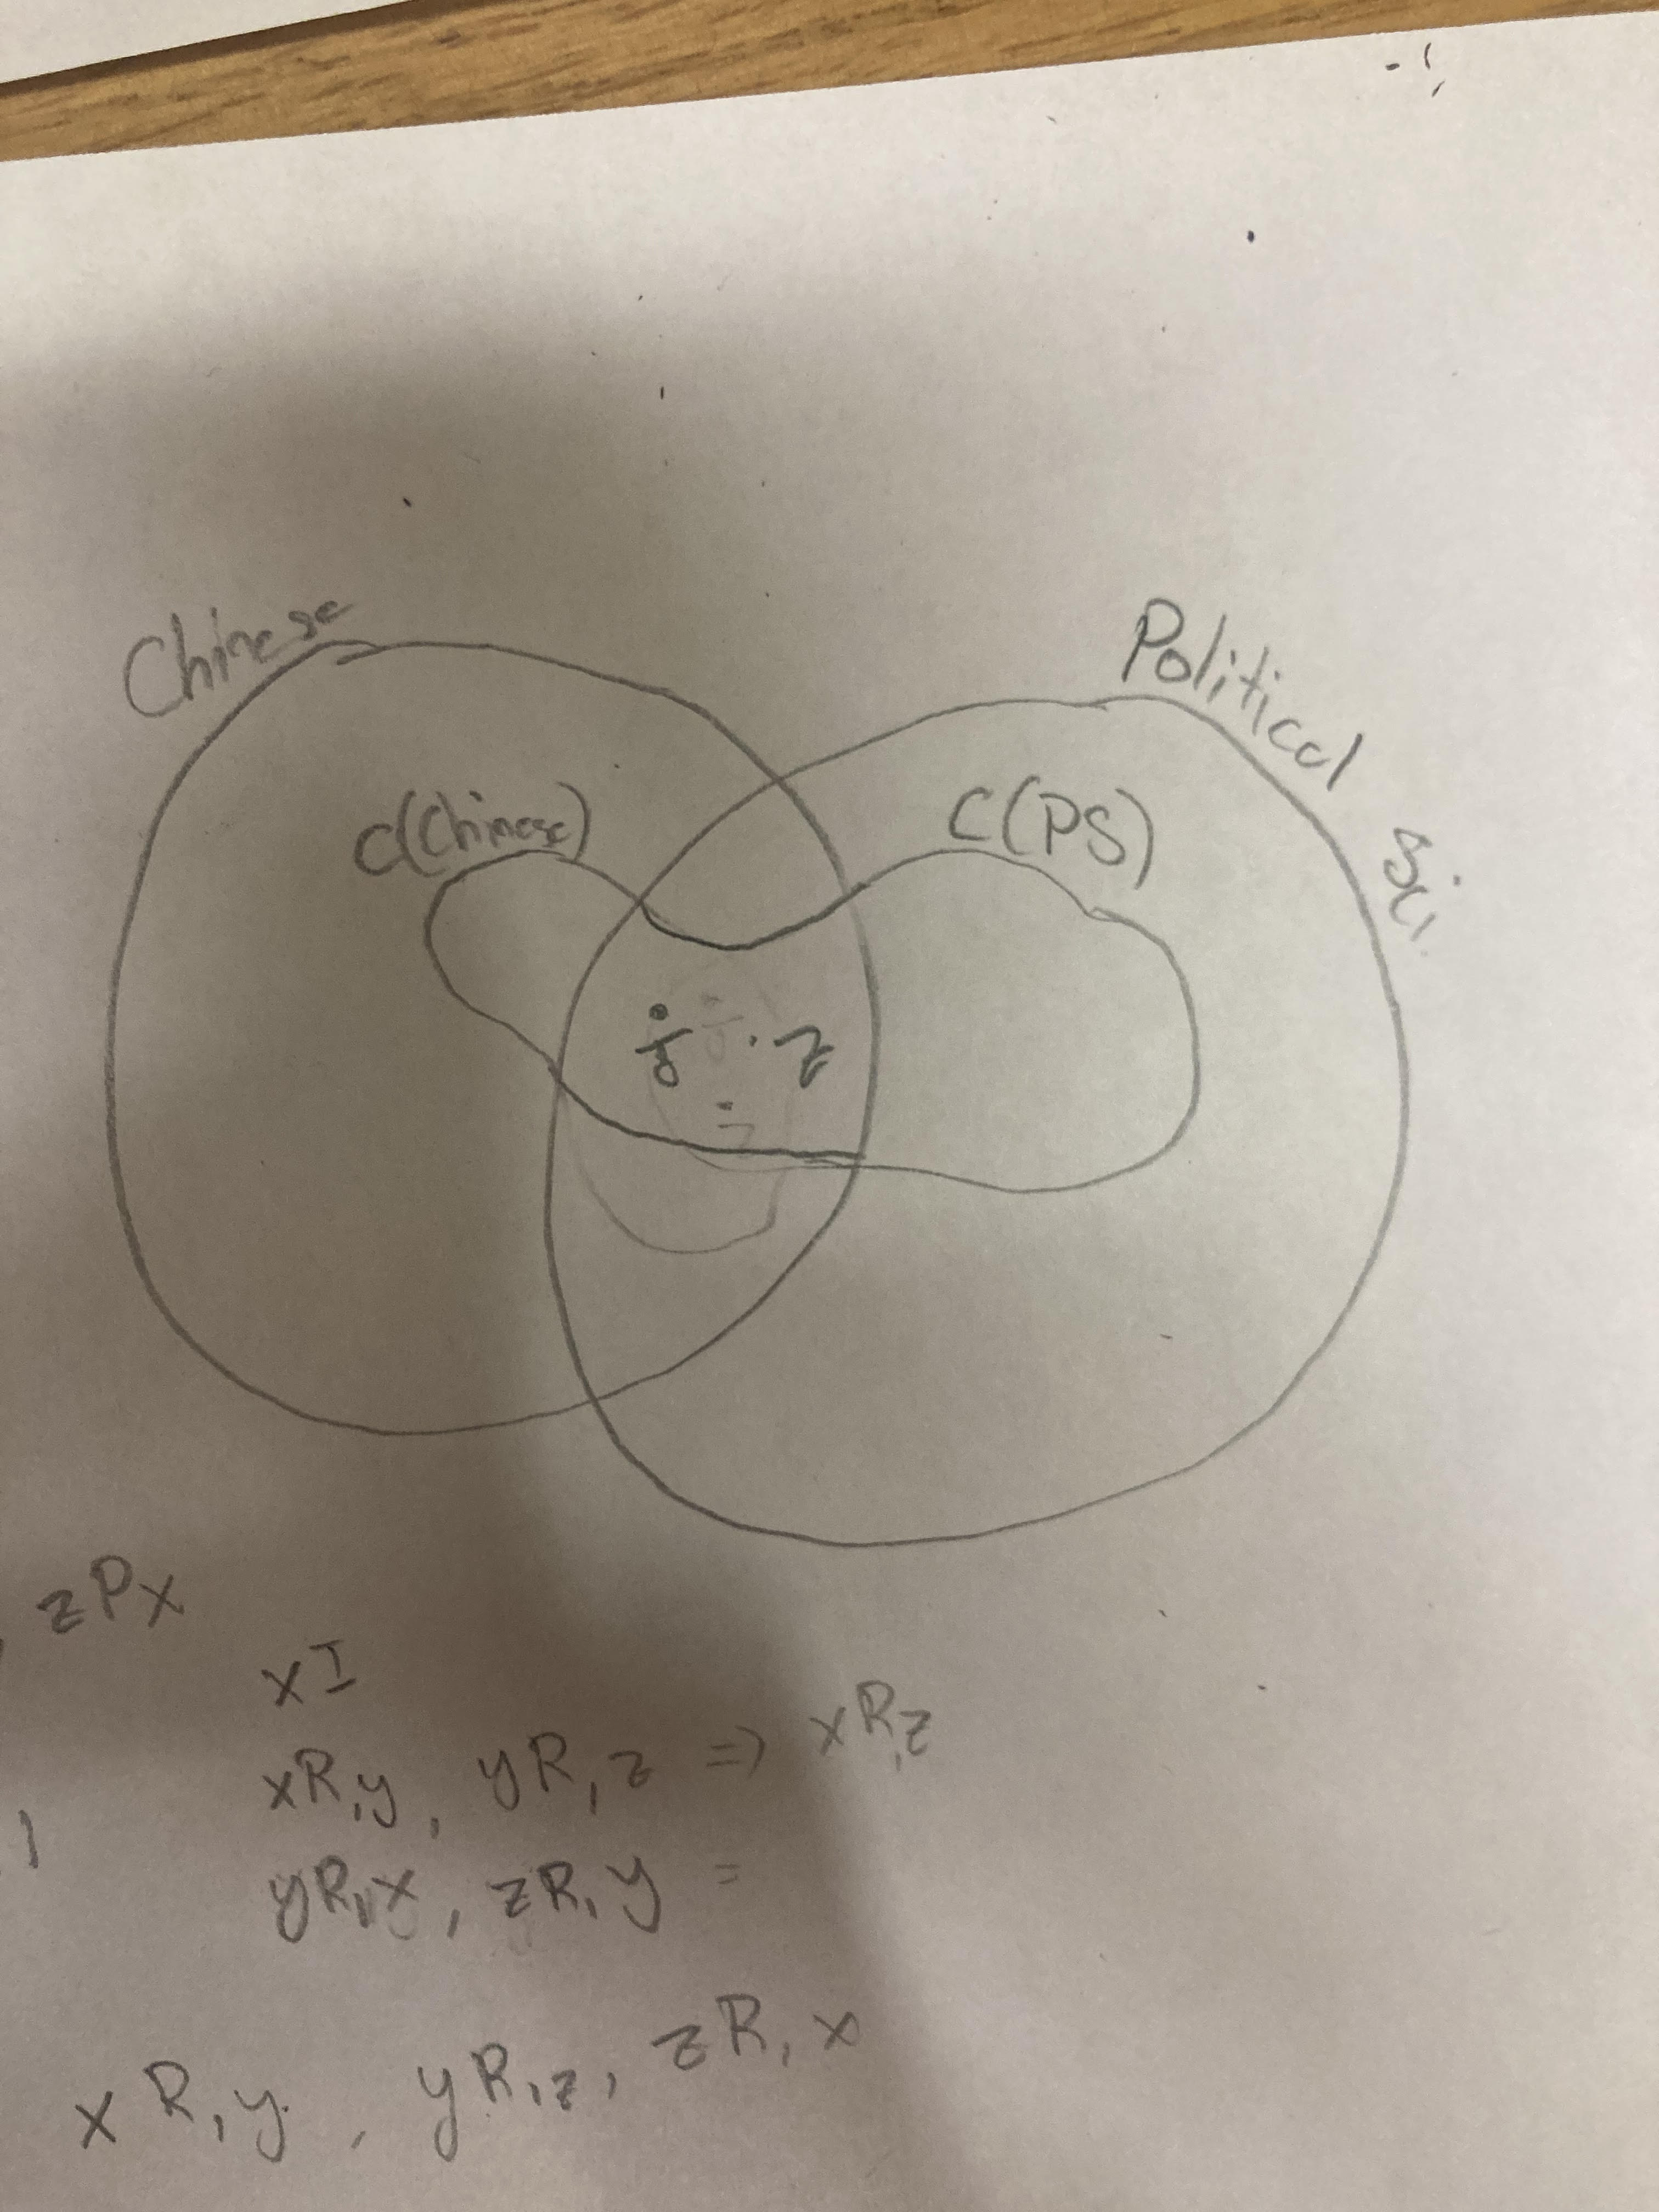
\includegraphics[width=0.5\linewidth]{Images/HW2.1.png}
        \caption{Venn Diagram}
    \end{figure}

    \item 
    \begin{problem}
        Show that if your preference satisfy WARP, the above statement must be true.
    \end{problem}
    \begin{solution}
        Suppose my preference satisfies WARP, but the above statement is not true. Thus, we have that $j \in C(CH)$ and $z\in C(PS),$ but either $j \notin C(PS)$ or $z \notin C(CH).$
        \begin{enumerate}
            \item Suppose $j\notin C(PS),$ then since $j \in PS,$ we have that $j \in PS\sm C(PS).$ We also have that $z \in C(PS)$ and $j \in C(CH),$ and thus by WARP $z\notin CH.$ Which is a contradiction since Juan is Chinese.
            \item An almost identical contradiction can be found for the other case.
        \end{enumerate}
        Thus, we have that that $j \in C(PS)$ and $z\in C(CH).$
    \end{solution}
\end{enumerate}

\newpage
\section*{Problem 2}
\begin{problem}
    Consider the following aggregation rules. Is each of the rules (1) transitive; (2) weakly Paretian; (3) non-dictatorial? Explain or give a counterexample.
\end{problem}
\begin{enumerate}
    \item 
    \begin{problem}
        Plurality: $aPb$ if $|i \in N \; ; \; aP_ib|> |i \in N \; ; \; bP_ia|$
    \end{problem}
    \begin{solution}:\\
        \begin{enumerate}
            \item \textbf{It is not transitive.} Suppose $X = \{x,y,z\}$ and $N=3$ with the following preference profiles:
            \[xP_1yP_1z\]
            \[yP_2zP_2x\]
            \[zP_3xP_3y\]
            Thus, we have that $2/3$ strictly prefer $x$ to $y,$ and thus $xPy.$ Similarly, we have that $yPz.$ However, we also have $zPx.$
        \item \textbf{It is weakly Paretian.} Suppose we have that for all $i\in N,$ $xP_iy.$ Thus we have that $|i \in N \; ; \; xP_i y| = N$ and $0 = |i \in N \; ; \; yP_i x|.$ Thus, by plurality we have that $xPy,$ satisfying weak Pareto.
        \item \textbf{It is non-dictatorial.} Let $N$ be the number of preference profiles and consider $X = \{x,y\}.$ If $xPy,$ then we must have that at least $\frac{N}{2} + 1$ chose $xP_iy.$ Thus, at most $\frac{N}{2} -1$ chose $yP_ix.$ Without loss of generality, one can change voters such that we have $yPx,$ and call that amount $k.$ Thus, we have that $k>\frac{N}{2}.$ Take the original voters of $yP_ix$ and move them to $xP_iy,$ then we have that $xPy$ again. Thus, there does not exist a single $i \in N$ that is in every decisive set. 
        \end{enumerate}
    \end{solution}
    \item 
    \begin{problem}
        Reverse dictatorship: 
        $\exists i \in N$ such that $\forall x,y, \; xP_iy \implies yPx$
    \end{problem}
    \begin{solution}:\\
        \begin{enumerate}
            \item \textbf{It is not transitive unless we can assume that the non-dictator only has strict preferences}. Suppose the latter, then suppose $xRy$ and $yRz,$ then we want to show that $xRz.$ Since $xRy,$ then $yP_ix,$ as we are assuming the non-dictator only has strict relations. Similarly, we have that $zP_iy.$ Thus, because $R_i$ is transitive, then 
            \[zP_iyP_ix \implies zP_ix \implies xPz \implies xRz.\]
            However, if we assume the non-dictator can choose whatever they want, then it is not transitive. Suppose $xRy$ and $yRz,$ then we want to show that $xPz.$ To do this, just let the non-dictator be indifferent with respect to $x$ and $z,$ and thus the group preference can be whatever it wants, including $xPz$ (i.e, if it is a simple majority if the dictator is indifferent or something then everyone not the non-dictator goes $xP_jz$)
            \item \textbf{It is not weakly Paretian.} Suppose that for all $i \in N,$ $xP_iy.$ Thus, we have that the reverse dictator has $xP_iy,$ and thus $yPx.$ 
            \item \textbf{It is not dictatorial.} There does not exist a $j\in N$ such that if $xP_jy$ then $xPy$ since we have that $xPy$ if and only if the dictator has $yP_ix$ 
        \end{enumerate}
    \end{solution}
    \item 
    \begin{problem}
        Roman Republican System: There exist two consuls $i, j.$ For any alternatives $x, y,$ If both $xP_iy$ and $xP_jy$, then the social preference is $xPy$. If not, the social preference
regarding $x$ and $y$ is decided by a simple majority vote of all citizens (including the two consuls)
    \end{problem}
    \begin{solution}
        \begin{enumerate}
            \item \textbf{It is not transitive.} Consider $X = \{x,y,z\}$ and let $N = \{1,2,3\}$ and let individuals $1$ and $2$ be the consuls. Suppose
            \[xP_1y, xP_2y, yP_3x \implies xPy\]
            \[yP_1z, zP_2y, yP_3z \implies yPz\]
            \[xP_1z, zP_2x, zP_3x \implies zPx,\] then we have that $P$ is not transitive.
            \item \textbf{It is Weakly Paretian.} Suppose that for all $i\in N,$ we have that $xP_iy.$ Thus, both of the consuls strictly prefer $x$ to $y,$ and thus $xPy.$
            \item \textbf{It is non-dictatorial.} Evidently, none of the non-consuls are dictators. Neither consul is a dictator since if the other votes opposite and the rest of $N$ agrees, then the group goes opposite this consul.
        \end{enumerate}
    \end{solution}
\end{enumerate}

\newpage
\section*{Problem 3}
There are three alternatives, i.e. $A = \{x, y, z\}$ and a group of two players $N =\{1, 2\}.$ Consider the following aggregation rule. Player 1 is almost the dictator with one
exception — player 2 can veto the possibility that $x$ be socially preferred to $y$. In other
words, the group preference adheres to citizen 1’s preference except the scenario when $xP_1y$
but $yP_2x$, in which case $xIy$, i.e. $x$ is socially indifferent to $y$. Show that this rule is acyclic, weakly Paretian, and IIA, but is not transitive.
\begin{solution}
\begin{itemize}
    \item (Acyclic)
    Suppose $xPy$ and $yPz,$ then we have that 
    \[xP_1y, xP_2y \qquad yP_1z, yP_2z.\] Notice that $P_2$ could be switched to $R_2$ or $I_2,$ but not a strict preference opposite of $1,$ but we suffer no loss of generality by assuming $P_2.$
    Since each individual has transitive preference relation, then 
    \[xP_1z, xP_2z \implies xPz\implies xRz.\] Thus, $R$ is acylic.\\
    \item (Weak Pareto) Suppose that for all $i\in N,$ we have that $xP_iy.$ This obviously implies $xPy$ since the dictator says so and $2$ is not against it. Thus, we have that $R$ is weakly Paretian.\\
    \item (IIA) Suppose that for some $\rho, \rho' \in R^n,$ we have that $\rho_{x,y} = \rho_{x,y}'.$ Thus, we have that the kinda dictator and $2$ have the same thoughts about $x$ and $y$ in both $\rho$ and $\rho'.$ Since the group preference only cares about their thoughts on $x$ and $y,$ then $f(\rho) = f(\rho').$ More formally, suppose $f(\rho)\neq f(\rho').$ The only interesting cases are the following:
    \[xIy, xP'y \quad \text{or} \quad xPy, xI'y.\]
    However, in the first case we must have that $2$ changed their opinions in $\rho',$ and thus $\rho' \neq \rho.$ Similarly for the second.
    \item (\textbf{Not} Transitive) Consider the following preference profile:
    \[xP_1yP_1z, \qquad yP_2xP_2z\] Thus, we have that 
    \[xIy, xPz, yPz,\] implying that $R$ is not QT, and thus not transitive. 
\end{itemize}
\end{solution}

\newpage
\section*{Problem 4}
\begin{problem}
    
Consider a society of $19 + x$ citizens with the following preferences over three candidates
$\{a, b, c\}$:
\begin{enumerate}
\item 10 citizens: $a P b P c;$
\item 5 citizens: $b P c P a;$
\item 4 citizens: $c P a P b;$
\item x citizens: $c P b P a;$
\end{enumerate}
\end{problem}

\begin{enumerate}
\item
\begin{problem}
        Suppose the election adopts the Borda rule. That is, a voter gives a score $1$ to their most preferred candidate, a $2$ to their second most preferred, and so on. Socially, the candidate with a lower total score is preferred to one with a higher total score. What
is the range of $x$ (the number of citizens with preferences $c P b P a$) that
\begin{enumerate}
\item makes a the Borda count winner?
\item makes b the Borda count winner?
\item makes c the Borda count winner?
\end{enumerate}
(If you think a candidate can never be a Borda winner regardless the value of x, please
also explain why.)
\end{problem}
\begin{solution}
Consider that $a$ has $f(n) = 33 + 3n$ trophies. $b$ has $g(n) = 37 + 2n,$ and $c$ has $h(n) = 44 + n.$
    \begin{enumerate}
        \item For $n<4,$ we have that $f(n) <g(n)$ and  $f(4) = 45 = g(4).$ Evidently, we have that $g(n)< h(n).$ Thus, $a$ has the least points and is thus chosen.
        \item For $n \in \{5,6\},$ we have that $g(n)< f(n)< h(n),$ and thus $b$ has the least amount of points.
        \item for $n>7,$ we have that $h(n)> f(n)< g(n),$ and thus $c$ has the least amount of points.
    \end{enumerate}
\end{solution}
\item 
\begin{problem}
    What is the range of $x$ that makes $c$ the Borda count winner but not the winner under a simple majority rule? (If you think such x does not exist, please also
explain why.)
\end{problem}
\begin{solution}
    For $x\geq 12,$ we have by the above that $c$ has the least number of points. Moreover, we have that $\frac{16}{31}> \frac{1}{2}$ voted for $c,$ and thus is the winner under simple majority. Thus, if $x \in \{8,9,10,11\},$ then $c$ is the Borda count winner but not the simple majority winner.
\end{solution}
\end{enumerate}

\newpage
\section*{Problem 5}
\begin{problem}
    Prove that if $f$ is a non-collegial simple rule, it must have at least three minimally decisive coalitions.
\end{problem}
\begin{solution}
Easy Proof: Since $f$ is a simple rule, then $s(f)\geq 3,$ where $s(\dot)$ is the Nakamura number. Thus, by the book definition of Nakamura number, is must have at least three minimally decisive sets\\

Alternate: Suppose $f$ has 1 minimally decisive coalition, the it must be collegial! Let $L_1$, $L_2 \in \mathcal{L}(f)$.
Then since $\mathcal{L}(f)$ is proper, $L_1 \cap L_2 \neq \emptyset$. Since this is true for
any $L_1$, $L_2 \in \mathcal{L}(f)$, it must be that $K(\mathcal{L}) \neq \emptyset$ when $|\mathcal{L}| = 2$ and $\mathcal{L}\subset \mathcal{L}(f).$ Thus, $|\mathcal{L}|\geq 3.$
\end{solution}

\newpage
\section*{Problem 6}
\begin{problem}
    Let the set of alternatives be $X = \{a,b,c\}$ and the set of agents be $N = \{1,2,3\}$. Suppose that society adopts a preference
aggregation rule that works in the following way. First, there is a simple majority
rule vote between $a$ and $b$. Second, there is a simple majority rule vote between
the winner of the first round and $c$. Let $x_1$ be the winner of the second round,
$x_2$ be the loser of the second round, and $x_3$ be the loser of the first round.
The social preference relation is then defined as $x_1 P x_2$, $x_2 P x_3$, and
$x_1 P x_3$. As mentioned in class, this is the rule adopted in the \textit{New
Zealand Flag Referendum} in 2015.
\begin{itemize}
\begin{problem}
\item Construct a preference profile that shows this preference aggregation rule is \textit{not} weakly Paretion.
\end{problem}
\begin{solution} Consider the following preference profile, $\rho$:
\begin{enumerate}
    \item Let $aP_1b$ and $aP_2b$ and $aP_3b.$
    \item Let $aP_1c$ and $aP_2c$ and $aP_3c.$
    \item Let $bP_1c$ and $bP_2c$ and $bP_3c.$
\end{enumerate}
The first round between $a$ and $c$ shows that $a$ wins, then the second round between $a$ and $c$ shows that $a$ wins. Thus, the social preference relation is $aPb$ $cPb$ and $aPb.$ However, Notice that $cPb,$ even though by (c) Weakly Paretian would imply that $bPc.$
\end{solution}
\begin{problem}
\item Construct a preference profile that shows this preference
aggregation rule is \textit{not} IIA.
\end{problem}
\begin{solution}
    Consider the following preference profile, $\rho'$:
    \begin{enumerate}
    \item Let $bP_1a$ and $bP_2a$ and $bP_3a.$
    \item Let $bP_1c$ and $bP_2c$ and $bP_3c.$
    \item Let $aP_1c$ and $aP_2c$ and $aP_3c.$
\end{enumerate}
Then $a$ loses the first round, $b$ wins the second. Thus, we have that $bPc$ and $bPa$ and $cPa.$ Thus, considering the preference profile from part (a) above, we have that $\rho|_{b,c} = \rho'|_{b,c}$ and $cPb$ but $bP'c.$
\end{solution}

\end{itemize}    

\end{problem}

\end{document}